\subsection{Access Control Lists}

We introduce access control lists to provide a generalized form of access
control through a well-understood and common interface:

\begin{enumerate}
  \item \sol{interface AccessControlList}, which defines the basic actions
    required for an access control list implementation;

  \item \sol{contract BasicACL}, which provides a basic implementation of
    \sol{interface AccessControlList}; and

  \item \sol{contract ACLAuthority}, which aggregates an
    \solt{interface AccessControlList} implementation, \sol{contract BasicACL}
    in this case, to back an \sol{interface Authority} implementation.
\end{enumerate}

\begin{figure}[H]
  \centering
  \figurepdf[]{access-control-lists}
  \caption{Generalized contract access control by way of access control lists.}\label{fig:acl}
  % 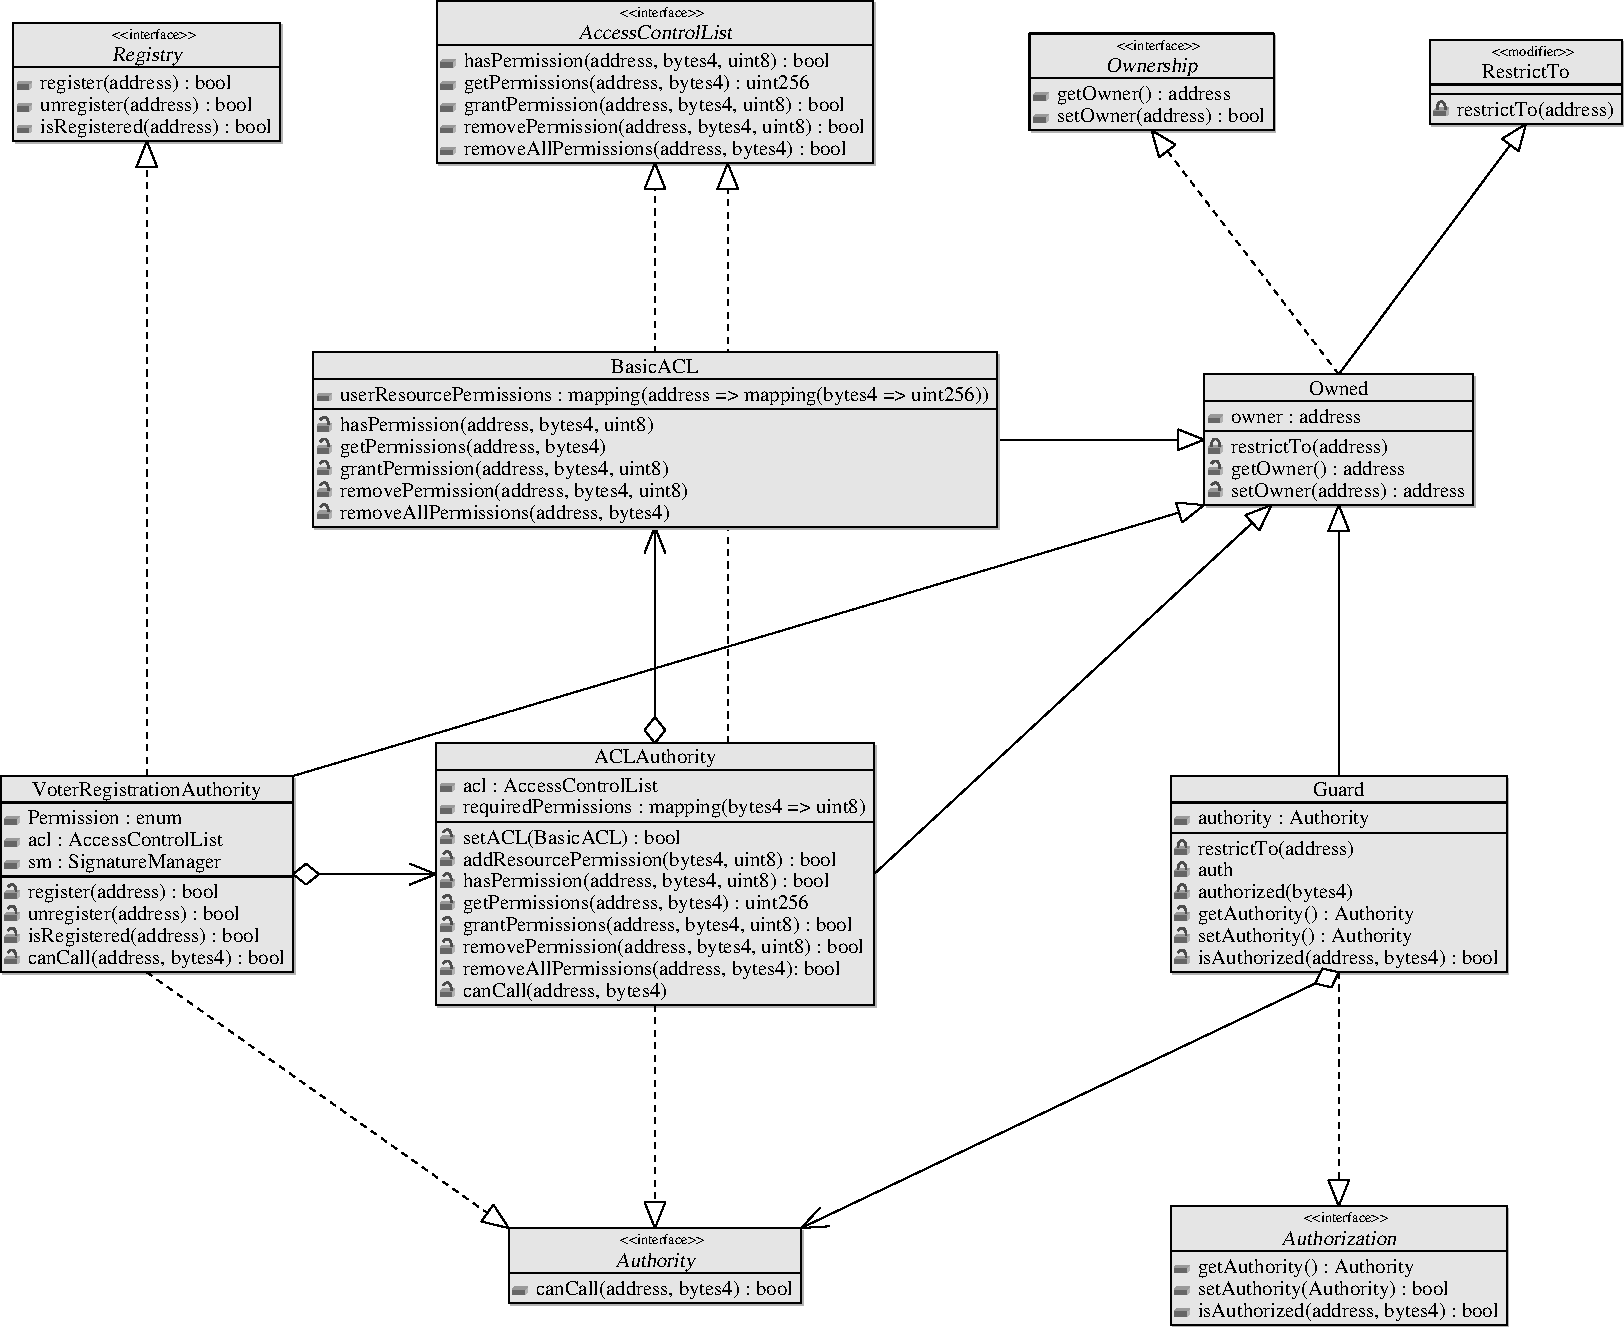
\includegraphics[width=\textwidth]{figures/authorization/figure}
  % \includestandalone[width=\textwidth]{\fig{authorization}}
\end{figure}

\subsubsection{Interface AccessControlList}

The \solt{interface}, \sol{interface AccessControlList}, introduces five
\solt{function} definitions to achieve basic access control list functionality:

\begin{enumerate}
  \item \sol{function hasPermission}, which validates that a \emph{subject} has
    the \emph{permission} required access some \emph{resource}.

  \item \sol{function getPermissions}, which returns the \emph{permissions} some
    \emph{subject} has for a given \emph{resource}.

  \item \sol{function setPermissions}, which updates the \emph{permissions} some
    \emph{subject} has for a given \emph{resource}.

  \item \sol{function grantPermission}, which grants a single \emph{permission}
    for some \emph{subject} with respect to some \emph{resource}.

  \item \sol{function revokePermission}, which revokes a single
    \emph{permission} for some \emph{subject} with respect to some
    \emph{resource}.
\end{enumerate}

\begin{solidity}[interface AccessControlList]
interface AccessControlList {
  function hasPermission (address _subject, bytes4 _resource, uint8 _permission)
    public view returns (bool _hasPermission);

  function getPermissions (address _subject, bytes4 _resource)
    public view returns (uint256 _permissions);

  function setPermissions (address _subject, bytes4 _resource, uint256 _permissions)
    public returns (bool _success);

  function grantPermission (address _subject, bytes4 _resource, uint8 _permission)
    public returns (bool _success);

  function revokePermission (address _subject, bytes4 _resource, uint8 _permission)
    public returns (bool _success);
}
\end{solidity}

\begin{interface}
  \begin{functions}
    \item \sol{function hasPermission (address _subject, bytes4 _resource, uint8 _permission)},
      evaluates whether some \emph{subject} has the requisite \emph{permission}
      to access some \emph{resource}.
      \begin{parameters}
        \item \sol{address _subject}, the \solt{address} of an account
          representing the \emph{subject}, i.e., the \emph{user}, to evaluate
          permissions against.
        \item \sol{bytes4 _resource}, the \emph{resource}, signature hash of a
          Solidity \solt{function}, to validate \emph{permissions} against.
        \item \sol{uint8 _permission}, a \emph{permission} level, or
          \emph{action}, which is being validated.
      \end{parameters}
      \begin{returns}
        \item \sol{bool _hasPermission}, returns the \solt{true} if the
            \emph{subject} has the requisite \emph{permission} to access the
            \emph{resource}, otherwise \solt{false}.
      \end{returns}

    \item \sol{function getPermissions (address _subject, bytes4 _resource)},
      retrieves the \emph{permissions}, for a \emph{<subject, resource>} pair.

      \begin{parameters}
        \item \sol{address _subject}, the account \solt{address} of the
          \emph{subject} whose \emph{permissions} are to be retrieved.

        \item \sol{bytes4 _resource}, the \emph{resource}, \solt{function}
          signature, which the \emph{permissions} should be retrieved for.
      \end{parameters}

      \begin{returns}
      \item \sol{uint256 _permissions}, the \solt{uint256} representation of the
        \emph{subject's} \emph{permissions} for a given \emph{resource}.
      \end{returns}

    \item \sol{function setPermissions (address _subject, bytes4 _resource, uint256 _permissions)},
      updates a \emph{subject's} \emph{permissions} for some \emph{resource}.

      \begin{parameters}
        \item \sol{address _subject}, the account \solt{address} of the
          \emph{subject} whose \emph{permissions} are to be modified.

        \item \sol{bytes4 _resource}, the \emph{resource}, \solt{function}
          signature, which the \emph{permissions} are to be modified for.

        \item \sol{uint256 _permissions}, the \solt{uint256} representation of
          the \emph{subject's} new \emph{permissions} for the \emph{resource}.
      \end{parameters}

      \begin{returns}
      \item \sol{bool _success}, resolves to \solt{true} if the operation was
        successful, otherwise \solt{false}.
      \end{returns}

    \item \sol{function grantPermission (address _subject, bytes4 _resource, uint8 _permission)},
      grants a \emph{subject} some \emph{permission} for a given \emph{resource}.

      \begin{parameters}
        \item \sol{address _subject}, the account \solt{address} of the
          \emph{subject} whose \emph{permissions} are to be modified.

        \item \sol{bytes4 _resource}, the \emph{resource}, \solt{function}
          signature, which the \emph{permissions} are to be modified for.

        \item \sol{uint8 _permission}, a \solt{uint8} value representing the
          \emph{permission-bit} to enable for the \emph{<subject, resource>}
          pair.
      \end{parameters}

      \begin{returns}
      \item \sol{bool _success}, resolves to \solt{true} if the operation was
        successful, otherwise \solt{false}.
      \end{returns}

    \item \sol{function revokePermission (address _subject, bytes4 _resource, uint8 _permission)},
      revokes a \emph{subject's} \emph{permission} for a given \emph{resource}.

      \begin{parameters}
        \item \sol{address _subject}, the account \solt{address} of the
          \emph{subject} whose \emph{permissions} are to be modified.

        \item \sol{bytes4 _resource}, the \emph{resource}, \solt{function}
          signature, which the \emph{permissions} are to be modified for.

        \item \sol{uint8 _permission}, a \solt{uint8} value representing the
          \emph{permission-bit} to revoke for the \emph{<subject, resource>}
          pair.
      \end{parameters}
      \begin{returns}
        \item \sol{bool _success}, resolves to \solt{true} if the operation was
          successful, otherwise \solt{false}.
      \end{returns}
  \end{functions}
\end{interface}

% \paragraph{function hasPermission}
%
% \subparagraph{Parameters}
% \begin{enumerate}
%   \item \sol{address _subject}, which represents some \emph{subject}, or
%         \emph{user}, accessing some \emph{resource}.
%   \item \sol{bytes4 _resource}, a \emph{resource}, or Solidity
%         \solt{function}, to validate \emph{permissions} against.
%   \item \sol{uint8 _permission}, a \emph{permission} level, or \emph{action},
%         which is being validated.
% \end{enumerate}
%
% \subparagraph{Returns}
% \sol{function hasPermission} is expected to \solt{return} a \solt{bool},
% \sol{bool _hasPermission}, which resolves to \solt{true} if the
% \emph{subject} has permission to access the \emph{resource}, Solidity
% \solt{function} associated with \sol{bytes4 _resource}, at the
% \emph{permission} level specified by \sol{uint8 _permission}.
%
% \paragraph{function getPermissions}
% \subparagraph{Parameters}
% \subparagraph{Returns}
%
% \paragraph{function setPermissions}
% \subparagraph{Parameters}
% \subparagraph{Returns}
%
% \paragraph{function grantPermission}
% \subparagraph{Parameters}
% \subparagraph{Returns}
%
% \paragraph{function removePermission}
% \subparagraph{Parameters}
% \subparagraph{Returns}
%


\subsubsection{Contract BasicACL}

The \solt{contract}, \sol{contract BasicACL}, implements the ACL
\solt{interface}, \sol{interface AccessControlList}, to provide a primitive
ACL implementation. The \solt{contract} implementation is backed by a mapping of
references, from \emph{subject} to \emph{resource} to \emph{permissions} --- as
described in Chapter~\ref{chap:methods}, \emph{\nameref{chap:methods}} --- i.e.,
a nested sparse vector mapping.

\begin{solidity}[contract BasicACL]
contract BasicACL is Owned, AccessControlList {
  mapping (address => mapping (bytes4 => uint256)) subjectResourcePermissions;

  function hasPermission (address _subject, bytes4 _resource, uint8 _permission) public constant restrictTo(owner) returns (bool _hasPermission) {
    uint256 result = subjectResourcePermissions[_subject][_resource] & (uint256(1) << _permission);
    return (result > 0);
  }

  function getPermissions (address _subject, bytes4 _resource) public constant restrictTo(owner) returns (uint256 _permissions) {
    return subjectResourcePermissions[_subject][_resource];
  }

  function grantPermission (address _subject, bytes4 _resource, uint8 _permission) public restrictTo(owner) returns (bool _success) {
    subjectResourcePermissions[_subject][_resource] |= uint256(1) << _permission;
    return true;
  }

  function revokePermission (address _subject, bytes4 _resource, uint8 _permission) public restrictTo(owner) returns (bool _success) {
    subjectResourcePermissions[_subject][_resource] &= ~(uint256(1) << _permission);
    return true;
  }

  function setPermissions (address _subject, bytes4 _resource, _permissions) public restrictTo(owner) returns (bool _success) {
    subjectResourcePermissions[_subject][_resource] = _permissions;
    return true;
  }
}
\end{solidity}

\begin{state}
  \begin{public}
    \item \sol{mapping (address => mapping (bytes4 => uint256)) subjectResourcePermissions}
      a nesting mapping used to record the \emph{permissions} which
      \emph{subjects} have to access various \emph{resources}.

      \begin{displayquote}
        Here \emph{subjects} are represented and identified by their account
        \solt{address}; \emph{resources} are assumed to be \solt{function}
        signatures, \solt{bytes4}; and \emph{permissions} are bit vectors,
        backed by \solt{uint256} values, where bit masks are leveraged to
        retrieve individual \emph{permission} values.
      \end{displayquote}
  \end{public}
\end{state}

\begin{code}
  \begin{functions}
    \item \sol{function hasPermission (address _subject, bytes4 _resource, uint8 _permission)},
      evaluates whether some \emph{subject} has the requisite \emph{permission}
      to access some \emph{resource}.

      \begin{displayquote}
        \emph{Permission} evaluation occurs by:
        \begin{enumerate}
          \item retrieving the \emph{permissions} bit vector from the
            \solt{mapping} \sol{subjectResourcePermissions}, where the
            \emph{subject}, \sol{address _subject}, and \emph{resource},
            \sol{bytes4 _resource}, are used as keys;

          \item creating a \emph{permission} bit mask by left-shifting 1
            \sol{_permission} times, \sol{1 << _permission};

          \item evaluating \sol{permissions |$\land$| bit_mask}; and finally,

          \item returning \solt{true} if the value resulting from the evaluation
            is greater than 0, i.e., the \emph{subject} has \emph{permission} to
            access to the \emph{resource}.
        \end{enumerate}
      \end{displayquote}

      \begin{parameters}
        \item \sol{address _subject}, the \solt{address} of an account
          representing the \emph{subject}, i.e., the \emph{user}, to evaluate
          permissions against.
        \item \sol{bytes4 _resource}, the \emph{resource}, signature hash of a
          Solidity \solt{function}, to validate \emph{permissions} against.
        \item \sol{uint8 _permission}, a \emph{permission} level, or
          \emph{action}, which is being validated.
      \end{parameters}

      \begin{returns}
        \item \sol{bool _hasPermission}, returns the \solt{true} if the
          \emph{subject} has the requisite \emph{permission} to access the
          \emph{resource}, otherwise \solt{false}.
      \end{returns}

    \item \sol{function getPermissions (address _subject, bytes4 _resource)},
      retrieves the \emph{permissions}, for a \emph{<subject, resource>} pair.

      \begin{parameters}
        \item \sol{address _subject}, the account \solt{address} of the
          \emph{subject} whose \emph{permissions} are to be retrieved.

        \item \sol{bytes4 _resource}, the \emph{resource}, \solt{function}
          signature, which the \emph{permissions} should be retrieved for.
      \end{parameters}

      \begin{returns}
      \item \sol{uint256 _permissions}, the \solt{uint256} representation of the
        \emph{subject's} \emph{permissions} for a given \emph{resource}.
      \end{returns}

    \item \sol{function setPermissions (address _subject, bytes4 _resource, uint256 _permissions)},
      updates a \emph{subject's} \emph{permissions} for some \emph{resource}.

      \begin{modifiers}
        \item \sol{modifier restrictTo (owner)}, restricts access to the
          \solt{function} such that \emph{only} the current \solt{owner} of the
          \solt{contract} can call it.
      \end{modifiers}

      \begin{parameters}
        \item \sol{address _subject}, the account \solt{address} of the
          \emph{subject} whose \emph{permissions} are to be modified.

        \item \sol{bytes4 _resource}, the \emph{resource}, \solt{function}
          signature, which the \emph{permissions} are to be modified for.

        \item \sol{uint256 _permissions}, the \solt{uint256} representation of
          the \emph{subject's} new \emph{permissions} for the \emph{resource}.
      \end{parameters}

      \begin{returns}
        \item \sol{bool _success}, resolves to \solt{true} if the operation was
          successful, otherwise \solt{false}.
      \end{returns}

    \item \sol{function grantPermission (address _subject, bytes4 _resource, uint8 _permission)},
      grants a \emph{subject} \emph{permission} for a given \emph{resource}.

      \begin{displayquote}
        \emph{Permission} grant occurs by:
        \begin{enumerate}
          \item retrieving the \emph{permissions} bit vector from the
            \solt{mapping} \sol{subjectResourcePermissions}, where the
            \emph{subject}, \sol{address _subject}, and \emph{resource},
            \sol{bytes4 _resource}, are used as keys;

          \item creating a \emph{permission} bit mask by left-shifting 1
            \sol{_permission} times, \sol{1 << _permission};

          \item evaluating \sol{permissions |$\lor$| bit_mask} to produce a new
            \emph{permissions} bit vector; and finally,

          \item updating the state of the \solt{contract} by storing the
            resulting \emph{permissions} bit vector back into the
            \sol{subjectResourcePermissions} \solt{mapping}.
        \end{enumerate}
      \end{displayquote}

      \begin{modifiers}
        \item \sol{modifier restrictTo (owner)}, restricts access to the
          \solt{function} such that \emph{only} the current \solt{owner} of the
          \solt{contract} can call it.
      \end{modifiers}

      \begin{parameters}
        \item \sol{address _subject}, the account \solt{address} of the
          \emph{subject} whose \emph{permissions} are to be modified.

        \item \sol{bytes4 _resource}, the \emph{resource}, \solt{function}
          signature, which the \emph{permissions} are to be modified for.

        \item \sol{uint8 _permission}, a \solt{uint8} value representing the
          \emph{permission-bit} to enable for the \emph{<subject, resource>}
          pair.
      \end{parameters}

      \begin{returns}
      \item \sol{bool _success}, resolves to \solt{true} if the operation was
        successful, otherwise \solt{false}.
      \end{returns}

    \item \sol{function revokePermission (address _subject, bytes4 _resource, uint8 _permission)},
      revokes a \emph{subject's} \emph{permission} for a given \emph{resource}.

      \begin{displayquote}
        \emph{Permission} revocation occurs by:
        \begin{enumerate}
          \item retrieving the \emph{permissions} bit vector from the
            \solt{mapping} \sol{subjectResourcePermissions}, where the
            \emph{subject}, \sol{address _subject}, and \emph{resource},
            \sol{bytes4 _resource}, are used as keys;

          \item creating a \emph{permission} bit mask by left-shifting 1
            \sol{_permission} times, \sol{1 << _permission};

          \item flipping all of the bits of the \emph{permission} bit mask,
            \sol{~bit_mask};

          \item evaluating \sol{permissions |$\land$| bit_mask} to produce a new
            \emph{permissions} bit vector; and finally,

          \item updating the state of the \solt{contract} by storing the
            resulting \emph{permissions} bit vector back into the
            \sol{subjectResourcePermissions} \solt{mapping}.
        \end{enumerate}
      \end{displayquote}

      \begin{modifiers}
        \item \sol{modifier restrictTo (owner)}, restricts access to the
          \solt{function} such that \emph{only} the current \solt{owner} of the
          \solt{contract} can call it.
      \end{modifiers}

      \begin{parameters}
        \item \sol{address _subject}, the account \solt{address} of the
          \emph{subject} whose \emph{permissions} are to be modified.

        \item \sol{bytes4 _resource}, the \emph{resource}, \solt{function}
          signature, which the \emph{permissions} are to be modified for.

        \item \sol{uint8 _permission}, a \solt{uint8} value representing the
          \emph{permission-bit} to revoke for the \emph{<subject, resource>}
          pair.
      \end{parameters}

      \begin{returns}
      \item \sol{bool _success}, resolves to \solt{true} if the operation was
        successful, otherwise \solt{false}.
      \end{returns}
  \end{functions}
\end{code}


\subsubsection{Contract ACLAuthority}

The \solt{contract}, \sol{contract ACLAuthority}, merges the ACL functionality
introduced by \sol{interface AccessControlList} with the generalized access
control functionality introduced by \sol{interface Authority}.

\begin{solidity}[contract ACLAuthority]
contract ACLAuthority is Owned, Authority, AccessControlList {
  AccessControlList acl;
  mapping (bytes4 => uint8) requiredResourcePermission;

  constructor (bool _createACL) {
    if (_createACL) acl = new BasicACL();
  }

  function hasPermission (address _subject, bytes4 _resource, uint8 _permission) public constant returns (bool _hasPermission) {
    return acl.hasPermission(_subject, _resource, _permission);
  }

  function getPermissions (address _subject, bytes4 _resource) public constant returns (uint256 _permissions) {
    return acl.getPermissions(_subject, _resource);
  }

  function grantPermission (address _subject, bytes4 _resource, uint8 _permission) public restrictTo(owner) returns (bool _success) {
    return acl.grantPermission(_subject, _resource, _permission);
  }

  function revokePermission (address _subject, bytes4 _resource, uint8 _permission) public restrictTo(owner) returns (bool _success) {
    return acl.removePermission(_subject, _resource, _permission);
  }

  function setPermissions (address _subject, bytes4 _resource, uint256 _permissions) public restrictTo(owner) returns (bool _success) {
    return acl.setPermissions(_subject, _resource, _permissions);
  }

  function setACL(AccessControlList _acl) public restrictTo(owner) returns (bool _success) {
    assert(_acl.owner() == address(this));
    acl = _acl;
    return true;
  }

  function setRequiredResourcePermission (bytes4 _resource, uint8 _permission) public restrictTo(owner) returns (bool _success) {
    requiredResourcePermission[_resource] = _permission;
    return true;
  }

  function canCall (address _subject, bytes4 _resource) public constant returns (bool _canCall) {
    return hasPermission(_subject, _resource, requiredResourcePermission[_sig]);
  }
}
\end{solidity}

\begin{state}
  \begin{public}
  \item \sol{AccessControlList acl} maintains the \solt{address} of an ACL
    implementation, a \solt{contract} which implements \sol{interface
    AccessControlList}.

  \item \sol{mapping (bytes4 => uint8) requiredResourcePermissions} maintains a
    mapping of \solt{function}[s], \sol{bytes4}, to required
    \emph{permission}, \sol{uint8}.
  \end{public}
\end{state}

\begin{code}
  \begin{constructor}
  \item \sol{constructor (bool _createACL)}, upon creation and initialization
    of this \solt{contract} the \solt{constructor} can deploy a
    \solt{contract}, \sol{contract BasicACL}, if the \solt{bool}, \sol{bool
    _createACL}, is set to \solt{true}.

    \begin{parameters}
    \item \sol{bool _createACL}, set to \solt{true} to deploy an ACL
      implementation, \sol{contract BasicACL}, in addition to this
      \solt{contract}; otherwise \solt{false}.
    \end{parameters}
  \end{constructor}

  \begin{functions}
  \item \sol{function setAcl (AccessControlList _acl)}, updates the
    \solt{contract} reference which is responsible for managing ACL requests.

    \begin{modifiers}
    \item \sol{modifier restrictTo (owner)}, restricts access to the
      \solt{function} such that \emph{only} the current \solt{owner} of the
      \sol{contract} can call it.
    \end{modifiers}

    \begin{parameters}
    \item \sol{AccessControlList _acl}, the ACL implementation which access
      control responsibilities are to be delegated to.
    \end{parameters}

    \begin{returns}
    \item \sol{bool _success}, resolves to \solt{true} if the operation was
      successful, otherwise \solt{false}.
    \end{returns}


  \item \sol{function setRequiredResourcePermission (bytes4 _resource, uint8 _permission)},
    updates the mapping representing the \emph{permission} required to access
    some \emph{resource}, \solt{function} signature.

    \begin{modifiers}
    \item \sol{modifier restrictTo (owner)}, restricts access to the
      \solt{function} such that \emph{only} the current \solt{owner} of the
      \sol{contract} can call it.
    \end{modifiers}

    \begin{parameters}
    \item \sol{bytes4 _resource}, the \emph{resource}, \solt{function}
      signature, which the \emph{permission} is to be modified for.

    \item \sol{uint8 _permission}, a \solt{uint8} value representing the
      \emph{permission-bit} required for the \emph{resource}.
    \end{parameters}

    \begin{returns}
    \item \sol{bool _success}, resolves to \solt{true} if the operation was
      successful, otherwise \solt{false}.
    \end{returns}


  \item \sol{function canCall (address _subject, bytes4 _resource)}, evaluates
    whether a \emph{subject} can access to some \emph{resource} by validating
    with the ACL implementation that the \emph{subject} has the required
    \emph{resource} \emph{permission}.

    \begin{parameters}
    \item \sol{address _subject}, the \emph{subject}, Ethereum account,
      whose \emph{permissions} are being evaluated.

    \item \sol{bytes4 _resource}, the \emph{resource}, \solt{contract
      function}, which the \emph{subject's} \emph{permissions} are being
      evaluated against.
    \end{parameters}

    \begin{returns}
    \item \sol{bool _canCall}, resolves to \solt{true} if the
      \emph{subject}, \sol{address _subject}, is permitted to access the
      \emph{resource}, \sol{bytes4 _resource}, otherwise \solt{false}.
    \end{returns}


  \item
    \sol{function hasPermission (address _subject, bytes4 _resource, uint8 _permission)}, \\
    \sol{function getPermissions (address _subject, bytes4 _resource)}, \\
    \sol{function setPermissions (address _subject, bytes4 _resource, uint256 _permissions)}, \\
    \sol{function grantPermission (address _subject, bytes4 _resource, uint8 _permission)}, \\
    \sol{function revokePermission (address _subject, bytes4 _resource, uint8 _permission)}, \\
    all ACL responsibilities originating from \sol{interface AccessControlList}
    are delegated to the provided ACL implementation stored in
    \sol{AccessControlList acl}.

    \begin{modifiers}
    \item \sol{modifier restrictTo (owner)}, restricts access to the
      \solt{function} such that \emph{only} the current \solt{owner} of the
      \solt{contract} can call this \solt{function}; this applies to
      \solt{function}[s] \sol{setPermissions}, \sol{grantPermission}, and
      \sol{revokePermission}.
    \end{modifiers}
  \end{functions}
\end{code}

